\documentclass[../main.tex]{subfiles}
    
\begin{document}
\doublespacing



\subsection{Variables}

\subfile{variables} % Subsection for Variables

\subsection{Hypothesis}
Firstly, if the Mpemba effect is to be observed then the initially hotter sample ($T = \SI{50}{\celsius}$) has to reach $\SI{0}{\celsius}$ before the initially cooler sample ($T = \SI{28}{\celsius}$). Secondly, if the salt concentration in tap water samples of $\SI{40}{\milli\liter}$ increases from $\SI{1.0}{\gram}$ to $\SI{5.0}{\gram}$, then the time taken for the samples to reach $\SI{0}{\celsius}$ will decrease, which might lead to the Mpemba effect being observed. \par

\subsection{Equipment}
In this study the following equipment was used:
\begin{singlespacing}
\begin{itemize}
    \item Small freezer with an internal temperature of $\SI{-20.1}{\celsius}$ to $\SI{-18.2}{\celsius}$
    \item Small plastic cups (PP05) measuring: top radius $(8.92 \pm 0.01 \si{\centi\meter})$, bottom radius $(6.21 \pm 0.01 \si{\centi\meter})$ and height $(9.76 \pm 0.01\si{\centi\meter})$
    \item Vernier caliper $(\SI{\pm 0.01}{\centi\meter})$
    \item Glass Beaker $(\SI{\pm 0.5}{\milli\liter})$
    \item Tap water
    \item Table salt
    \item Scale $(\SI{\pm 0.01}{\gram})$
    \item Arduino Uno Rev3 \autocite{arduino}
    \item Insulated temperature probe (NTC Thermistor) 
    \item Resistor with nominal resistance $\SI{1}{\kilo\ohm}$
    \item Paper towels
    \item Digital data logger (Laptop)
\end{itemize}
\end{singlespacing}

\subsection{Experimental Methods}

In this experiment, $\SI{40}{\milli\liter}$ samples of regular tap water were used with additionally added table salt (\SI{1.0}{\gram} - \SI{5.0}{\gram}) with increments of $\SI{1.0}{\gram}$. Water samples without additional salt were used as a control. To obtain the experimental data, an Arduino was set up and programmed to calculate the temperature of a thermistor. \par

\subsubsection{Setup}

Arduino was set up to collect relevant data and determine the potential difference of a thermistor. This was achieved by creating a voltage-divider over a regular $\SI{1}{\kilo\ohm}$ resistor (experimentally $\SI{989}{\ohm}$) and a $\SI{10}{\kilo\ohm}$ thermistor depicted on Fig.~\ref{fig:circuitDrawing}. Thermistor's specifications were experimentally found as shown in Table \ref{tab:resistorCharacteristics}. The circuit was completed and $\SI{5}{\volt}$ potential difference established over the circuit by using Arduino's $\SI{5}{\volt}$ and GND (Ground) ports as shown below. \par
\begin{figure}[H]
\centering
\begin{minipage}{.49\textwidth}
  \centering
  \captionsetup{justification=centering}
  \begin{circuitikz}[scale=1, european] 
        \draw (4,4) to[short, *-o] (0,4) node[anchor=east] {5V};
        \draw (4,4) to[R, l=$10^3\ \si{\ohm}$] (4,2); % Resistor
        \draw (4,2) to[short, *-o] (6,2) node[anchor=west] {A0};
        \draw(4,2) to[R, label={$R_T$}] (4,0); % Thermistor
        \draw (4,0) to[short, *-o] (0,0) node[anchor=east] {GND};
    \end{circuitikz}
    \caption{Circuit of resistor and thermistor $R_T$ connected to Arduino's analog port (A0)}
    \label{fig:circuitDrawing}
\end{minipage}%
\begin{minipage}{.49\textwidth}
  \centering
  \captionsetup{justification=centering}
  \begin{tabular}{cc}
        \toprule
        \textbf{Temperature} $\mathbf{\left(\si{\celsius}\right)}$ & \textbf{Resistance} $\mathbf{\left(\si{\ohm}\right)}$ \\
        (\SI{\pm 0.1}{\celsius}) & (\SI{\pm 1}{\ohm}) \\
        \midrule
        $22.6$ & $1330$\\
        $11.3$ & $2140$\\
        $9.5$  & $2320$\\
        $-13.7$& $7070$\\
        \bottomrule
    \end{tabular}
  \captionof{table}{Values of $R_T$ at \\specific temperatures}
  \label{tab:resistorCharacteristics}
\end{minipage}
\end{figure}

From Fig. \ref{fig:circuitDrawing}, the circuit has a resistance $R_{tot} = R + R_T$, where $R$ is resistor with nominal resistance $\SI{1}{\kilo\ohm}$ and $R_T$ is the thermistor. From this it follows that the voltage of the thermistor, $V_T$, can be easily by using the Ohm's Law as (see Appendix for derivation):
\begin{equation}
    V_T= V_{arduino} \cdot \frac{R_T}{R + R_T}.
\end{equation}

In order to establish a relationship between resistance and temperature, calibration of the thermistor was done by using the Steinhart-Hart $\beta$ equation \autocite{steinhart_calibration_1968}. By doing so, the voltage data was could processed in real-time using the Python code (refer to the Appendix) thereby returning the temperature of the sample. \par

\subsubsection{Procedure}
Initially, the \SI{40}{\milli\liter} samples of tap water were boiled and salt was added. After mixing the samples with salt, they were left rest for a few minutes and then placed into the freezer.

All samples were positioned \emph{approximately} in the center of the freezer and thermally insulated by paper towels to prevent frosting with freezer floor. This was done to account for the freezer's efficiency as well as  of the subsequent trials

The ambient temperature of the freezer was allowed to drop back to $\SI{-20}{\celsius}$ after every measurement according to Ibekwe \& Cullerne (2016). Briefly, the experiment was conducted in the following steps:

\begin{enumerate}
    \item Using a scale, $\SI{1.0}{\gram}$ of table salt was measured and placed into a plastic cup. For subsequent measurements, table salt was measured in $\SI{1.0}{\gram}$ increments in the range $\SI{1.0}{\gram}$ - $\SI{5.0}{\gram}$
    \item Tap water was heated up until the boiling point by using a kettle. (Kettle was previously thoroughly cleaned so as not to contain any source of impurities) 
    \item Boiled tap water was then sampled (\SI{40}{\milli\liter}) using a glass beaker and transferred into the same plastic cup
    \item Plastic cup was hand-stirred until the table salt completely dissolved and left to rest for a few minutes at room temperature
    \item When the sample reached \SI{50}{\celsius}, thermistor was placed in the middle of the sample, approximately \SI{1}{\centi\meter} from the surface level.
    \item Sample with the thermistor was then placed approximately in the center of the freezer and the data collecting process on the laptop started. (Freezer floor was insulated by using paper towels)
    \item Sample was left in the freezer until it reached $\SI{-5}{\celsius}$ (prompted by Python program), when the measuring stopped and sample was taken out.
    \item After the procedure had been repeated for all mass concentrations, almost identical procedure was done with the $\SI{28}{\celsius}$ (These samples were let to cool down to $\SI{28}{\celsius}$ after which they were placed in the freezer with the thermistor) 
\end{enumerate}

% No explaining things here: give a rundown of how the experiment was conducted.

% \subsubsection{Pilot Experiment}
% In the conducted pilot experiment an attempt was made to use $\SI{80}{\milli\liter}$ water samples instead of $\SI{40}{\milli\liter}$ ones. Using the thermistor and Arduino, with a sampling rate of $\SI{0.5}{\hertz}$, graph at Fig. \ref{fig:pilotStudy@80} was obtained for a control sample without additionally added salt.

% \begin{figure}[H]
%     \centering
%     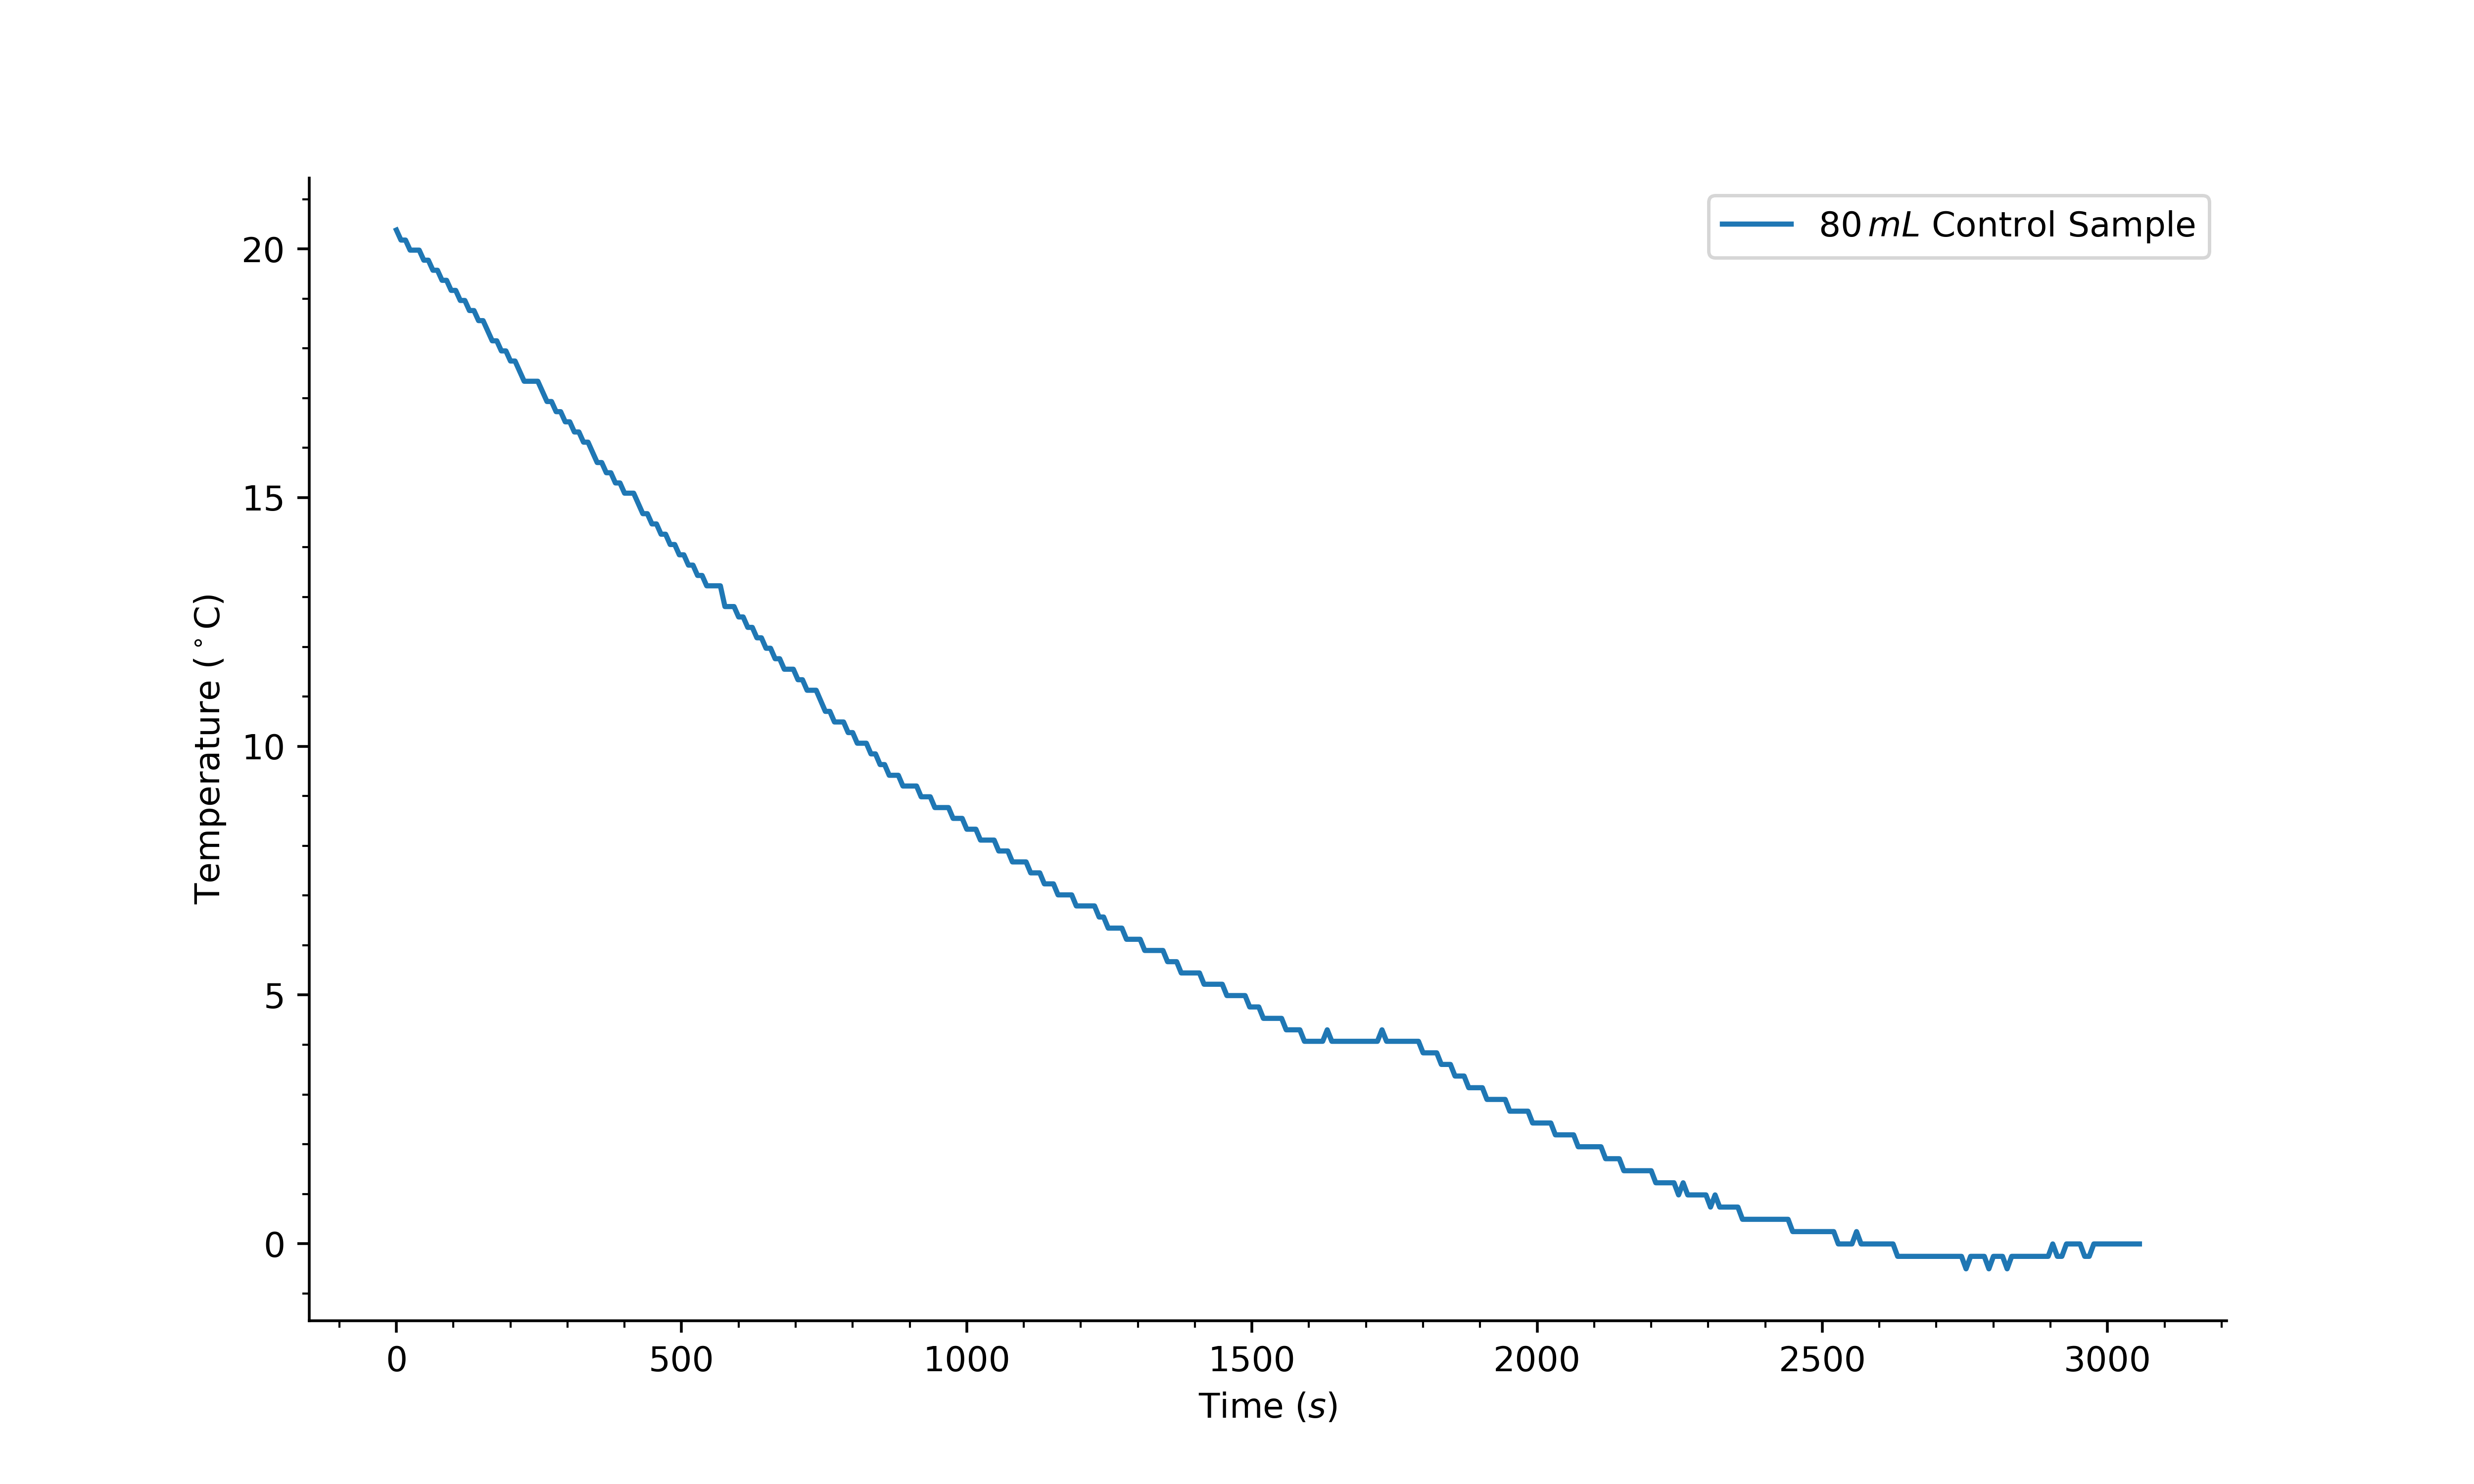
\includegraphics[scale=0.7]{figures/figurePilot80.png}
%     \caption{Control Sample of $(\SI{80}{\milli\liter})$ in the pilot experiment}
%     \label{fig:pilotStudy@80}
% \end{figure}

% Considering the graph in Fig.~\ref{fig:pilotStudy@80}, however, it may be noted that such sampling rate was too high. This sampling rate, together with a resolution of Arduino's analog-to-digital converter ($10$ bit) \autocite{noauthor_analogread_nodate} resulted in a step-wise function on a graph. This is to say that no significant changes in temperature occurred every $\SI{2}{\second}$ seconds. In addition to that, $\SI{80}{\milli\liter}$ sample proved to take longer to cool down, as expected because of the greater volume of water. To that end, in the subsequent measurements $\SI{40}{\milli\liter}$ samples were used and sampling rate was changed to $\SI{0.1}{\hertz}$. \par

\subsubsection{Safety Considerations}

During the experiment trials, special care was taken while handling hot water samples in order to avoid hand burn. As a precautionary measure, heat-resisting gloves were used. Similarly, when handling cooled samples the same gloves were used. No other biological or environmental hazards were identified.

\end{document}